\section{第二问的计算结果与扩散机制}
\label{q2-results}

\subsection{温度、含水率与空间差异}
表\ref{tab:q2-temperature}和表\ref{tab:q2-moisture}给出题目规定的
半小时间隔结果，均由式\eqref{q2-eq-richardson}的未舍入场保留四位小数得到。
逐秒工作簿\texttt{result2.xlsx}保存相同时域内21个半径位置的全部状态，
共$10800\times21\times2=453600$个结果。
\input{tables/q2_temperature}
\input{tables/q2_moisture}

至$3\unit{h}$，轴心和表面温度分别为49.8495\celsius、49.9664\celsius，
径向温差缩小至0.1169\unit{K}；轴心和表面含水率分别为1.7662、
1.0081\unit{kg/kg}，两者仍相差0.7581\unit{kg/kg}。
图\ref{q2-fig-profiles}显示，前半小时失水主要发生在外层，随后含水率变化向内部发展；
温度剖面则逐渐趋于平缓。这支持本时段热响应较快、水分分布仍显著不均匀的判断，
不能据此将药材含水率视为空间常数。

\begin{figure}[htbp]
\centering

\includegraphics[width=\textwidth]{figures/q2_profiles.pdf}
\caption{第二问不同时刻的中截面径向分布：左为温度，右为干基含水率；曲线对应0.5至3\unit{h}每隔0.5\unit{h}的结果。}
\label{q2-fig-profiles}
\end{figure}

圆柱中截面的平均状态必须按面积权重计算，
\begin{equation}
 \overline u(t)=\frac{2}{R^2}\int_0^R r u(r,t)\,\mathrm dr,
 \qquad u\in\{T,C\}.
\label{q2-eq-average}
\end{equation}
由此得$3\unit{h}$平均温度49.9043\celsius、平均含水率
1.3825\unit{kg/kg}。含水率积分较初态减少45.7833\%，
该比例表示固定参考干密度下的有效水分减少，不是由实测称量得到的失重率。
不能用21个等间隔半径节点的算术平均替代式\eqref{q2-eq-average}。

图\ref{q2-fig-history}进一步显示，表面较早响应环境，内部随后升温和失水。
第二问$0.5\unit{h}$轴心温度32.1892\celsius，低于第一问同一时刻的结果；
这是从初态采用不同物性所致，而非状态衔接错误。
第二问初始有效热容量更大，扩散系数还随温度变化，两问不能共用一段预热轨迹。

\begin{figure}[htbp]
\centering
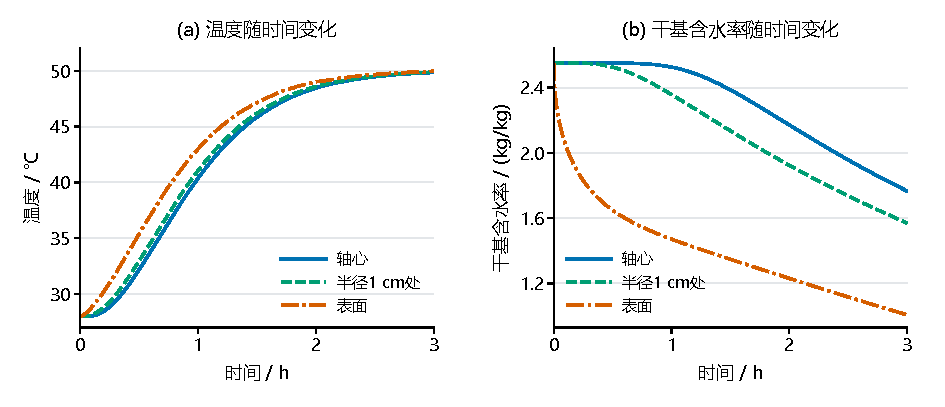
\includegraphics[width=\textwidth]{figures/q2_history.pdf}
\caption{轴心、半径1\unit{cm}及表面的状态历程：左为温度，右为干基含水率，使用前3\unit{h}的每秒状态。}
\label{q2-fig-history}
\end{figure}

\subsection{数值精度与几何近似的检验}
最初$1\unit{s}$的表面边界层对水分离散精度要求较高，
仅检查半小时论文表不足以保证逐秒文件可靠。
表\ref{q2-tab-verification}将空间误差、时间误差及独立实现比较分开列示。
固定$N=1280$时，减半容差并将最大步长降至$5\unit{s}$，
所得差异明显小于空间离散差异。
正式外推场与独立直接径向谱离散、Radau积分结果在全部453600个输出上
按实际四位小数格式逐值一致，两张论文表60个值亦一致。
第一秒表面含水率的正式未舍入值约为2.5198051473\unit{kg/kg}，显示为2.5198。

\begin{table}[htbp]
\centering\small
\caption{第二问的主要数值对照：规定逐秒径向采样上的最大绝对差}
\label{q2-tab-verification}
\begin{tabularx}{\textwidth}{@{}Xrr@{}}
\toprule
对照项目 & 温度/\unit{K} & 含水率/\unit{kg/kg}\\
\midrule
$N=1280$有限体积与192阶谱参考 & $4.1407\times10^{-7}$ & $7.9865\times10^{-5}$\\
$N=2560$有限体积与192阶谱参考 & $1.0333\times10^{-7}$ & $1.9903\times10^{-5}$\\
固定$N=1280$收紧时间容差与步长 & $7.6286\times10^{-10}$ & $7.1370\times10^{-11}$\\
正式外推场与独立径向谱--Radau解 & $1.3836\times10^{-9}$ & $1.1461\times10^{-7}$\\
\bottomrule
\end{tabularx}
\end{table}

原始$N=2560$解仍有个别数值跨越四位舍入边界，
故不能省略Richardson步骤后声称所有输出保持相同四位结果。
质量收支比较体积加权含水率变化与边界通量时间积分，
最大残差约$6.51\times10^{-12}\unit{kg/kg}$。
有效热收支比较$\int\!\int_V S(C)T_t\,\mathrm dV\mathrm dt$与侧面热输入，
相对残差约$3.11\times10^{-11}$；它不等于计算
$\int_V S(C)T\,\mathrm dV$的末初差，也不包含未建模的相变和携焓。

另以二维轴对称耦合模型检查本时段端部影响，在侧面和端面采用相同交换系数，
并与相同径向网格的一维模型配对。$40\times80$区间情景中，
中截面最大温度差约$1.70\times10^{-3}\unit{K}$、含水率差约
$2.25\times10^{-5}\unit{kg/kg}$。该结果支持前$3\unit{h}$中截面的径向近似，
但不保证几何简化后所有四位数字均不变，也不是数天时段或端面局部场的误差界。

\subsection{升温促进与失水抑制的竞争}
为解释扩散率随时间变化的原因，将式\eqref{q2-eq-properties}相对初态取对数，得
\begin{equation}
 \ln\frac{D(t,r)}{D_0}=H(t,r)+M(t,r),\qquad
 \begin{aligned}
 H&=3850\left(\frac{1}{301.15}-\frac{1}{T_K(t,r)}\right),\\
 M&=0.45\left(\frac{1}{2.55}-\frac{1}{C(t,r)}\right).
 \end{aligned}
\label{q2-eq-log-decomposition}
\end{equation}
初始$D_0=5.64168037\times10^{-9}\unit{m^2/s}$。
$H$和$M$分别度量相对初态的温度、含水率对数贡献，是沿耦合轨迹的严格代数分解，
不是冻结另一变量所得的反事实变化，也不是独立的因果贡献百分比。
按既定浮点表达式，在三个位置的逐秒样点上，恒等式重构残差不超过
$2.81\times10^{-15}$，仅用于核对代数重构，不作为PDE离散误差界。

\begin{figure}[htbp]
\centering

\includegraphics[width=\textwidth]{figures/q2_mechanism.pdf}
\caption{局部扩散率的累计变化：左为三位置$D/D_0$，右为表面温度项$H$、含水率项$M$及其和；右图各项为累计对数贡献，不是瞬时变化率。}
\label{q2-fig-mechanism}
\end{figure}

\begin{table}[htbp]
\centering\small
\caption{3\unit{h}的扩散率分解及最后半小时的净变化}
\label{q2-tab-mechanism}
\begin{tabular}{@{}rrrrr@{}}
\toprule
半径/cm & $H$ & $M$ & $D/D_0$ & $D(3\unit{h})/D(2.5\unit{h})-1$\\
\midrule
0 & 0.864803 & $-0.078317$ & 2.195668 & $-1.0612\%$\\
1 & 0.865730 & $-0.110117$ & 2.128916 & $-1.3937\%$\\
2 & 0.869116 & $-0.269903$ & 1.820685 & $-3.1596\%$\\
\bottomrule
\end{tabular}
\end{table}

图\ref{q2-fig-mechanism}与表\ref{q2-tab-mechanism}表明，
至$3\unit{h}$三位置的累计升温促进均大于累计失水抑制；
但表面扩散率在早期先下降，每秒采样的最小值出现在$144\unit{s}$，
$D/D_0=0.983282$。随后扩散率上升，轴心、1\unit{cm}和表面的
采样最大值分别出现在8856、8678、7262\unit{s}。
最后半小时，三个位置的$H$仍增加，而$M$降低的幅度更大，因而$D$净下降。
这些是有限时段和采样轨迹的结论，不意味着峰值之后每秒都由同一项占优。

若研究瞬时竞争，还需区分
\begin{equation}
 \partial_t\ln D=
 \underbrace{\frac{3850}{T_K^2}T_t}_{G_T}
 +\underbrace{\frac{0.45}{C^2}C_t}_{G_C}.
\label{q2-eq-rate}
\end{equation}
环境波动可能使$T_t$和$G_T$暂时为负，因此温度项并非每时每刻都促进扩散。
瞬时量用不跨越$60\unit{s}$输入折点的五点差分，并比较1、2、5\unit{s}间距；
初始边界层及接近零的导数仅作诊断，不赋予四位精度。
极小正含水率增量也不直接解释为实质吸湿。正文采用更稳健的区间净变化
说明阶段竞争，而不以局部导数符号代替全过程干燥瓶颈判断。
\FloatBarrier
